\chapname = {MAAS in VENV - II}

\chapter{\the\chapname}

In this chapter we will discuss the steps required to create a basic MAAS based virtual cloud environment. Remember that the problem statement is to repurpose the commodity hardware to create an experimental cloud. At present we don't have access to those hardwares hence we are conducting our experiments in a virtualized environment. 

\section{Creating an Isolated Network}

MAAS uses DHCP and DNS with PXE boot to enlist the nodes, so naturally you could have a conflict if you deploy this on a network with an existing DHCP server. Hence create a new (virtual) network with the following given steps from the QEMU interface:

\begin{enumerate}
    \setlength\itemsep{0em}
    \item Network name - maasisotest
    \item Disable DHCP configuration
    \item Choose IPv4 address which is not in use by any other connected network. I prefer to use 10.17.17.0/24.
    \item Select forwarding to physical network option and set destination to any physical device and mode to NAT
\end{enumerate}

The network configuration for 'maasisotest' should look similiar to Fig. 4.1. 

\begin{figure}[!ht]
    \centering
    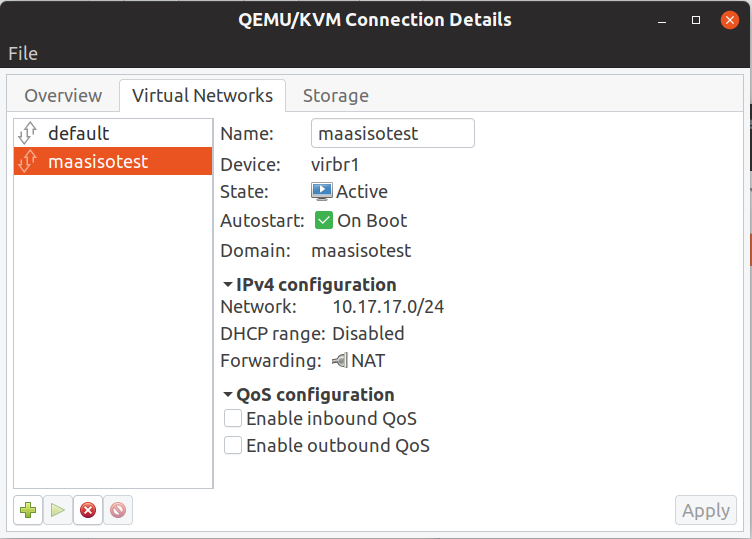
\includegraphics[width=0.5\textwidth]{images/4-1.png}
    \caption{Isolated network configuration}
\end{figure}

This will essentially create a router at the edge of this virtual network.

\section{Creating a maas controller}

Configurations for creating a new virtual machine with ubuntu 18.04 server installation. This machine will act as controller for the maas nodes.

\begin{itemize}
    \setlength\itemsep{0em}
    \item Memory - 1536 MB
    \item CPU Cores - 3
    \item Storage - 20 GB qcow2 
    \item Name - maas-controller
    \item Network - maasisotest
    \item NIC Interface 
    \begin{itemize}
        \item Network source - maasisotest
        \item Device model - virtio
    \end{itemize}
    \item Disk bus - virtio
    \item Remove unnecessary virtual hardware from the list for eg. sound
\end{itemize}

\begin{figure}[!ht]
    \centering
    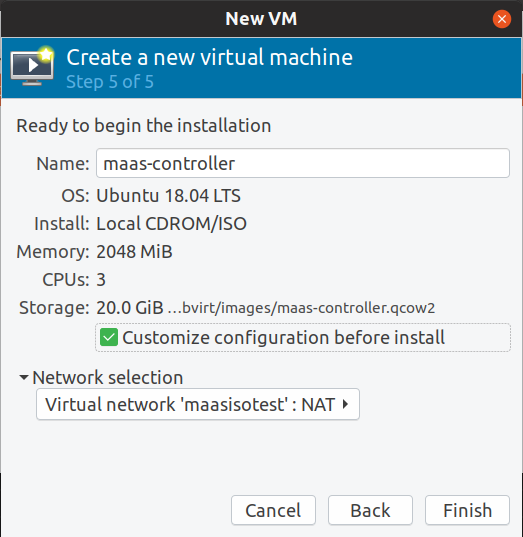
\includegraphics[width=0.5\textwidth]{images/4-2.png}
    \caption{maas-controller configuration}
\end{figure}

The basic configuration for maas-controller should look similar to Fig. 4.2.

Once the configuration is done we can proceed to installation.

\section{Installating ubuntu server image}

During the installation it is expected that DHCP acquisition will fail, since there is no DHCP server on that network. Hence, we need to configure this manually with a statiic IP address.

\begin{figure}[!ht]
    \centering
    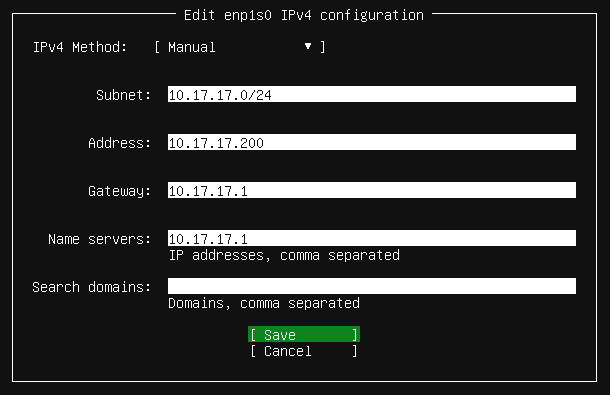
\includegraphics[width=0.5\textwidth]{images/4-3.png}
    \caption{IPv4 configuration}
\end{figure}

Kindly refer to the Fig. 4.3 for the IPv4 configuration. 

